\documentclass{article}
\usepackage[UTF8]{ctex}
\usepackage{amsmath,amssymb,amstext,amsfonts,mathtools}	%数学排版
\usepackage{graphicx,subfig}							%图形排版
\usepackage{array,multirow,makecell,diagbox}			%表格排版
\usepackage[table]{xcolor}
\usepackage{multicol,float}								%双栏排版
\usepackage{indentfirst}								%段落缩进
\usepackage{textcomp,bm,mathrsfs}						%字体
\usepackage[colorlinks=true,linkcolor=blue,filecolor=magenta,urlcolor=cyan]{hyperref}							%交叉引用
\usepackage{cleveref}
\usepackage{seqsplit}
\usepackage{titlesec}
\usepackage[tc]{titlepic}
\usepackage{cite}
\usepackage{booktabs}
\usepackage[section]{placeins}
\usepackage[a4paper,scale=0.8]{geometry}
\usepackage{fancyhdr}
\usepackage{microtype}
\usepackage{listings}
\usepackage{metalogo}

\setcounter{section}{-1}
\numberwithin{equation}{section}						%公式按章节编号
\numberwithin{figure}{section}							%图表按章节编号

\definecolor{dkgreen}{rgb}{0,0.6,0}
\definecolor{gray}{rgb}{0.5,0.5,0.5}
\definecolor{mauve}{rgb}{0.58,0,0.82}
\lstset{frame=tb,
	language=python,
	xleftmargin=2em,xrightmargin=2em,aboveskip=1em,belowskip=1em,
	showstringspaces=true,
	columns=fullflexible,
	linewidth=1\linewidth, %设置代码块与行同宽
	breaklines=true,%在单词边界处换行
	basicstyle={\small\ttfamily},
	numbers=left,
	%numberstyle=\tiny\courier, %设置行号大小
	numberstyle=\tiny\color{gray},
	keywordstyle=\color{blue},
	commentstyle=\color{dkgreen},
	stringstyle=\color{mauve},
	breaklines=true,
	breakatwhitespace=true,
	escapeinside=``,%逃逸字符(1左面的键),用于显示中文例如在代码中`中文...`
	tabsize=4,
	extendedchars=false %解决代码跨页时,章节标题,页眉等汉字不显示的问题
}
\pagestyle{fancy}

\fancyhead[L]{中国科学技术大学}
\fancyhead[C]{数学建模}
\fancyhead[R]{马祥超 \quad 姜一夫  \quad 胡泷}
\fancyfoot[C]{\thepage}

\newcommand{\upcite}[1]{\textsuperscript{\cite{#1}}}
\renewcommand{\dblfloatpagefraction}{.9}

\titleformat*{\section}{\center\bfseries\Large}
\titleformat*{\subsection}{\bfseries\large}

\title{{\heiti\huge{数码相机定位}}}
\author{\large{马祥超,姜一夫,胡泷}\\(中国科学技术大学,物理学院,合肥 230000)}
\date{\today}

\begin{document}
\begin{sloppypar}
	\thispagestyle{empty}
	\begin{center}
		\parbox[t][3cm][c]{\textwidth}{
		\begin{center}
				{\kaishu\Huge 中国科学技术大学}
		\end{center}}
		\parbox[t][8cm][c]{\textwidth}{\huge
		\begin{center} 
				\begin{figure}[H]
					\centering
					
\includegraphics[width=0.4\linewidth]{ustcblue}
				\end{figure}
		\end{center} }
		\parbox[t][2cm][t]{\textwidth}{
		\begin{center}  
				{\kaishu\huge 《数学建模》\\结课论文(2024春)}
		\end{center} }
		
		\parbox[t][5cm][b]{0.7\textwidth}{
			{\Large\kaishu{学生姓名 1:马祥超 \qquad\qquad\quad 学号:PB21020557\\
					学生姓名 2:姜一夫 \qquad\qquad\quad 学号:PB21020706\\
					学生姓名 3:胡泷  \quad\qquad\qquad\quad 学号:PB21051037\\
					Email 1:mc2003811@mail.ustc.edu.cn\\
					Email 2:jiangxianchen@mail.ustc.edu.cn\\
					Email 3:ustc\_hs@mail.ustc.edu.cn} }  }
		
		\parbox[t][5cm][c]{\textwidth}{ {\large
		\begin{center}
					{\Large\heiti 独立完成声明}
					\\
					本设计根据课程要求阅读材料并认真思考,独立撰写,严格杜绝学术不端行为。
		\end{center} } }
	\end{center}
	\clearpage
	\maketitle
	
	\noindent{\heiti{摘\quad 要:}\\}
	
	\noindent{\heiti{关键词:}}
	\newpage\tableofcontents\newpage
	\section{前言}

	\section{问题重述}
	\subsection{问题背景}
	随着计算机技术的发展,计算机视觉作为计算机科学技术的一个分支在近二十多年来也得到了迅猛发展和广泛应用,它用光学或电子器件模拟生物视觉的某些功能,获得被测物的信息,完成对三维信息的实时检测。视觉传感器是检测系统的核心部分,是系统获取数据的直接来源,对于视觉传感器而言,最重要的是通过二维图像获取物体在实空间的位置信息,而这就需要一些算法计算求解。
	\subsection{问题回顾}
	现有一个标定板,使用相机在不同角度拍摄若干照片,通过照片中的信息确定实空间中标定板各个点的三维点坐标。
	\section{问题分析}
	本问题的整体思路是:在仅已知物平面和像平面,相机的其他属性参数未知的前提下,建立相机模型,确定物平面上的点到像平面的像坐标的映射关系,其中包括照相机成像系统内外几何及光学参数的标定,从而达到只要给定若干像坐标上的点,就可直接通过模型求得其实坐标的目的。
	
	在具体建立照相机模型时,由于照相机与小孔成像在成像原理上没有本质区别,因此沿用现有比较成熟的摄机标定技术的理论思想。根据假设,靶标和像平面的图形是已知的,利用小孔成像原理建立模型,引入常用的相机模型坐标体系,确定各坐标体系的转换关系,建立线性相机模型,利用透视变换矩阵的相机标定技术的思想给出算法,求取相机模型的内部参数和外部参数,并将相机坐标系下的点转换位世界坐标系下的点。
	
	流程图如下:
	\begin{figure}[H]
		\centering
		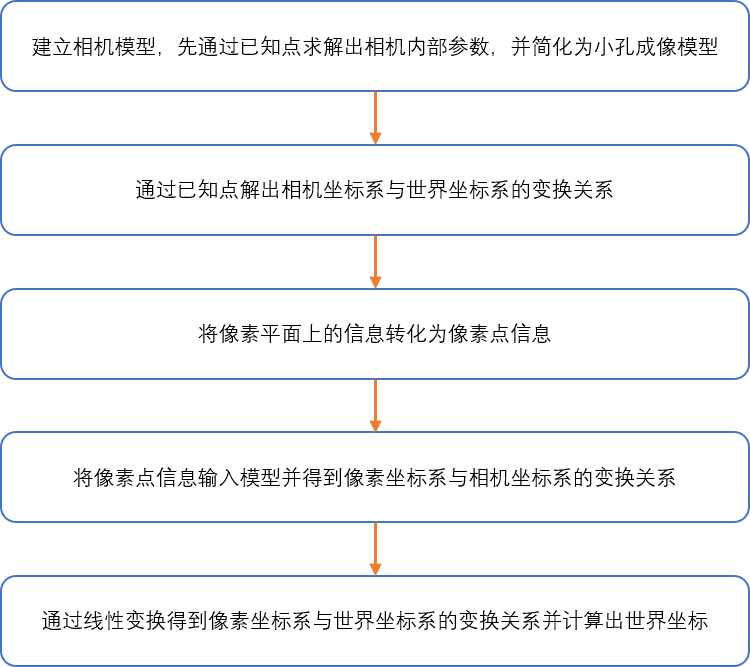
\includegraphics[width=0.7\linewidth]{flow_chart}
		\caption{求解问题流程图}
		\label{flow_chart}
	\end{figure}
	
	至此,我们已经有了解决问题的大致思路,接下来考虑如何建立模型。
	\section{基本假设}
	为了建立一个可行的模型,需要对其进行一些合理的假设.以下是对模型提出的假设或近似条件:
	\begin{enumerate}
		\item 假设使用的相机镜头没有非线性的畸变;
		\item 假设像平面上相邻的像素中心的横向与纵向距离相同;
		\item 假设像平面中心不存在偏移;
		\item 假设物平面与像平面中心与镜头的光学中心都在同一条光轴上;
		\item 像素的横纵间距都相等;
	\end{enumerate}
	\section{符号说明}
	对于接下来模型所要涉及的符号作如下说明:
	\begin{table}[H]
		\centering
		\begin{tabular}{c|c}
			\hline\hline
			数学符号 & 符号说明 \\ \hline
			${\bm X} = (X, Y, Z)^T$ & 世界坐标系下的一点 \\ 
			${\bm Y} = (x, y, z)^T$ & 像平面坐标系下一点 \\ 
			${\bm x} = (u, v, f)^T$ & 相机坐标系下一点 \\ 
			$f$ & 相机镜头的焦距 \\
			$O$ & 坐标系原点 \\
			${\bm R}$ & 旋转变换矩阵 \\ 
			${\bm T}$ & 平移变换向量 \\
			${\bm K}$ & 中心映射变换矩阵 \\
			${\bm A}$ & 相机内部标定矩阵 \\
			\hline
		\end{tabular}
	\end{table}
	\section{模型的建立}
	\subsection{小孔成像原理}
	当上述基本假设条件满足时,相机成像的光学原理可以使用最简单的小孔成像模型来刻画。
	
	小孔成像原理可表述为:将相机位置设为原点 $O$,物体表面上任一点 $\bm Y$,经连接点 $\bm Y$ 与原点的直线投射到像平面上 $\bm x$,从而构成物体的像.针孔对应于相机的光学中心,像平面与光心的距离称为有效聚焦长度或像距。
	
	取相机的光学中心为原点,以光轴为 $z$ 轴方向指向被摄物体,$x$,$y$ 轴分别平行于相片边框并构成右手坐标系.设像距为 $f$ 像平面方程为 $z=-f$ 作像关于原点的等距对称,得到平面 $z=f$ 上的图像我们不妨将 $z=f$ 视作像平面,而将 $z=-f$ 上的像在 $z=f$ 上的对称图像视作物体的像,如图 \ref{zuobiao}。
	\begin{figure}[H]
		\centering
		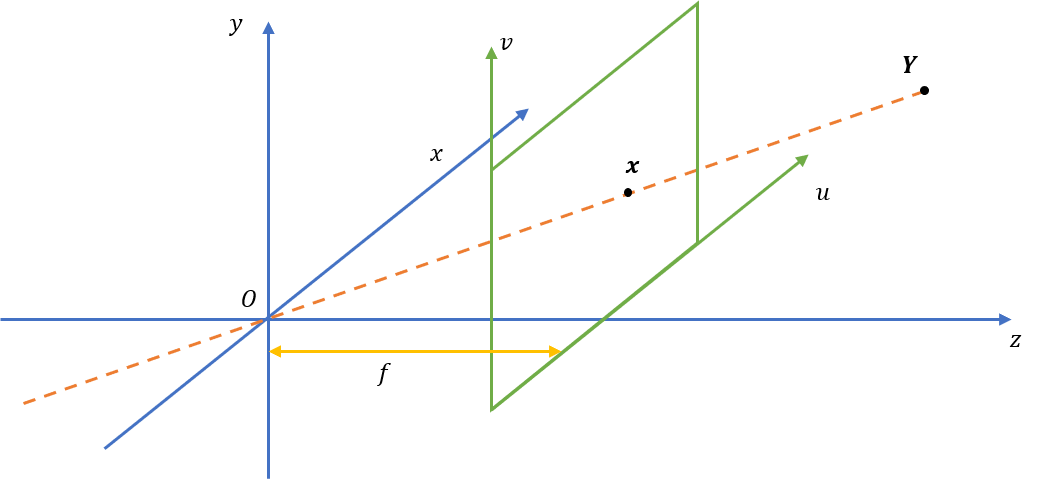
\includegraphics[width=0.8\linewidth]{zuobiao}
		\caption{小孔成像原理图示}
		\label{zuobiao}
	\end{figure}
	
	设点 $\bm Y$ 的坐标为 $(x,y,z)$,其像 $\bm x$ 的坐标为 $(u,v,f)$,因为实平面与像平面相平行且相似,则有式 \ref{eq1}
	\begin{equation}
		{\bm Y} = k{\bm x}
		\label{eq1}
	\end{equation}
	其中 $k = z/f$ 为比例系数,据上式则可以得到具体形式 \ref{eq2}
	\begin{equation}
		\left\lbrace
		\begin{aligned}
			&u = \frac{fx}{z} \\
			&v = \frac{fy}{z} \\
			&f = f
		\end{aligned}
		\right. 
		\label{eq2}
	\end{equation}
	
	取两个像素中心的距离作为长度单位(称为像素单位),令相片中心为像平面的原点,则 \ref{eq1} 式可视作物体到像平面的成像映射关系。
	
	式 \ref{eq1} 也可写为矩阵形式如式 \ref{eq1.1}
	\begin{equation}
		{\bm Y} = {\bm K}{\bm x}
		\label{eq1.1}
	\end{equation}
	其中
	\begin{equation}
		{\bm K} = \left(
		\begin{aligned}
			z/f,\ 0,\ 0 \\
			0,\ z/f,\ 0 \\
			0,\ 0,\ z/f
		\end{aligned}
		\right) 
	\end{equation}
	\subsection{双目定位的原理}
	现在我们来建立双目定位的数学模型.有两部相机,按照上一节的方法分别建立两部相机的相机坐标系.设空间任意一点在第一部相机的相机坐标系中的坐标为 ${\bm Y^1} = (x^1, y^1, z^1)^T$,而同一点在第二部相机的相机坐标系中的坐标为 ${\bm Y^2}=(x^2, y^2, z^2)^T$。假设已知两部相机的相对位置,即已知 ${\bm R}, {\bm T}$,坐标变换关系为式 \ref{eq3}
	\begin{equation}
		{\bm Y^1} = {\bm R}{\bm Y^2} + {\bm T}
		\label{eq3}
	\end{equation}
	其中
	\begin{equation}
		{\bm R} = \left( 
		\begin{aligned}
			r_{11},\ r_{12},\ r_{13} \\
			r_{21},\ r_{22},\ r_{23} \\
			r_{31},\ r_{32},\ r_{33}
		\end{aligned}
		\right), \quad {\bm T} = \left(
		\begin{aligned}
			t_{1} \\
			t_{2} \\
			t_{3}
		\end{aligned}
		\right)
	\end{equation}
	
	设同一点在两部相机中像平面坐标下分别为 ${\bm x^1} = (u^1, v^1, f)^T$ 和 ${\bm x^2} = (u^2, v^2, f)^T$,假设两个相机焦距相等,我们可以据式 \ref{eq1.1} 确定该点在两个相机坐标系中的坐标
	\begin{equation}
		\left\{
		\begin{aligned}
			{\bm Y^1} = {\bm K^1}{\bm x^1} \\
			{\bm Y^2} = {\bm K^2}{\bm x^2}
		\end{aligned}
		\right.
	\end{equation}
	具体形式如式 \ref{eq4}
	\begin{equation}
		\left\{
		\begin{aligned}
			{\bm Y^1} = z^1(\frac{u^1}{f}, \frac{v^1}{f}, 1)^T \\
			{\bm Y^2} = z^2(\frac{u^2}{f}, \frac{v^2}{f}, 1)^T
		\end{aligned}
		\right.
		\label{eq4}
	\end{equation}
	可以将解出的坐标 $\bm Y^1$ 与 $\bm Y^2$ 代入式 \ref{eq3} 这是关于 $\bm Y^1$ 和 $\bm Y^2$ 的超定方程,从中可以解出 $\bm Y^1$ 和 $\bm Y^2$,这就实现了该点的定位。
	
	在实际应用中,我们往往不止需要定位一个点,可能有许许多多的点,在两个相机坐标系下分别为 ${\bm Y^1_1}, {\bm Y^1_2}, \dots, {\bm Y^1_n}$ 与 ${\bm Y^2_1}, {\bm Y^2_2}, \dots, {\bm Y^2_n}$,这时从像素平面上得到点 ${\bm x^1_1}, {\bm x^1_2}, \dots, {\bm x^1_n}$ 与 ${\bm x^2_1}, {\bm x^2_2}, \dots, {\bm x^2_n}$ 的坐标,然后类似上述过程,列出方程组如下
	\begin{equation}
		\left\{
		\begin{aligned}
			&{\bm Y^1_i} = {\bm K^1}{\bm x^1_i} \\
			&{\bm Y^2_i} = {\bm K^2}{\bm x^2_i} \\
			&{\bm Y^1_i} = {\bm R_i}{\bm Y^2_i} + {\bm T_i}
		\end{aligned}
		\right. \qquad i = 1, 2, 3, \dots, n
	\end{equation}
	这时只需要解 $n$ 个超定方程即可。
	\subsection{相机相对位置的确定}
	在实际使用时,使用以相机为原点的坐标系可能不太方便,我们希望确定目标点在某个固定在地面的坐标系中的坐标,即世界坐标系,只要知道其中一部相机在世界坐标系中的相对位置,再通过一个坐标变换,就可实现。
	
	而且从上一节的讨论可以看到,要实现双目定位,确定两部相机的相对位置是关键。确定两部相机的相对位置就是要确定两部相机的相机坐标系之间的坐标变换关系。这一过程按相机定位的术语称为定位系统的外部参数标定外部参数标定的想法是引入世界坐标系,利用已知点在相机坐标系和世界坐标系之间的对应关系,决定相机坐标系和世界坐标系之间的变换。
	
	先研究一个相机坐标系与世界坐标系之间的坐标变换关系.设空间一点在世界坐标系和相机坐标系中的坐标分别为 ${\bm X_i} = (X_i, Y_i, Z_i)^T$ 和 ${\bm Y_i} = (x_i, y_i, z_i)^T$。
	
	取若干点,它们的世界坐标是已知的。用该相机拍摄后得到它们像的像素坐标为 ${\bm x_i} = (u_i, v_i, f)^T$,由中心射影变换式 \ref{eq1} 可得它们的相机坐标 ${\bm Y_i} = (x_i, y_i, z_i)$,设坐标变换关系为
	\begin{equation}
		{\bm Y} = {\bm R}{\bm X} + {\bm T}
		\label{eq5}
	\end{equation}
	其中
	\begin{equation}
		{\bm R} = \left( 
		\begin{aligned}
			r_{11},\ r_{12},\ r_{13} \\
			r_{21},\ r_{22},\ r_{23} \\
			r_{31},\ r_{32},\ r_{33}
		\end{aligned}
		\right), \quad {\bm T} = \left(
		\begin{aligned}
			t_{1} \\
			t_{2} \\
			t_{3}
		\end{aligned}
		\right)
	\end{equation}
	
	接下来需要用已知世界坐标系的点求出 ${\bm R}$ 与 ${\bm T}$,为方便考虑,取世界坐标系 $Z = 0$ 的点计算,由式 \ref{eq5} 得到
	\begin{equation}
		{\bm Y_i} = {\bm R}{\bm X_i} + {\bm T_i} \ \Rightarrow \
		\left\lbrace
		\begin{aligned}
			\frac{u_iz_i}{f} = r_{11}X_i + r_{12}Y_i + t_1 \\
			\frac{v_iz_i}{f} = r_{21}X_i + r_{22}Y_i + t_2 \\
			z_i = r_{31}X_i + r_{32}Y_i + t_3
		\end{aligned}
		\right.
	\end{equation}
	将第三个等式代如前两个得到
	\begin{equation}
		\left\lbrace
		\begin{aligned}
			u_i(r_{31}X_i + r_{32}Y_i + t_3) = f(r_{11}X_i + r_{12}Y_i + t_1) \\
			v_i(r_{31}X_i + r_{32}Y_i + t_3) = f(r_{21}X_i + r_{22}Y_i + t_2)
		\end{aligned}
		\right. \quad i = 1, 2, \dots, n
	\end{equation}
	而且已知 $\bm R$ 为旋转变换矩阵,即正交矩阵,满足正交条件
	\begin{equation}
		{\bm R}{\bm R^T} = {\bm I}
	\end{equation}
	
	将上面两式联立,只要 $n$ 足够大就可以求得 ${\bm R}$ 与 ${\bm T}$,即求出相机坐标系与世界坐标系的变换关系。
	
	对于双目定位的情形,设点在两个相机坐标系中的坐标分别为 ${\bm Y^1} = (x^1, y^1, z^1)$ 与 ${\bm Y^2} = (x^2, y^2, z^2)$,用以上的方法可以分别得到两个相机坐标系与世界坐标系的变换如下式
	\begin{equation}
		\left\lbrace
		\begin{aligned}
			{\bm Y^1} = {\bm R^1}{\bm X} + {\bm T^1} \\
			{\bm Y^2} = {\bm R^2}{\bm X} + {\bm T^2}
		\end{aligned}
		\right.
	\end{equation}
	可以得到两相机之间的坐标变换为
	\begin{equation}
		{\bm Y^1} = {\bm R}{\bm Y^2} + {\bm T}
	\end{equation}
	其中
	\begin{equation}
		{\bm R} = {\bm R^2}{\bm R^1}^T, \quad {\bm T} = {\bm T^2} - {\bm R^2}{\bm R^1}^T{\bm T^1}
	\end{equation}
	\subsection{多目定位的原理}
	在实际情况中,由于相机镜头非线性畸变、像平面中心偏移等问题,使用双目定位可能会有各种各样的误差,故而引入多目定位,即相机有多个,设在 $i$ 个相机坐标系相平面的 $j$ 个点坐标为 ${\bm x^i_j}$,如图 \ref{duomu},
	\begin{figure}[H]
		\centering
		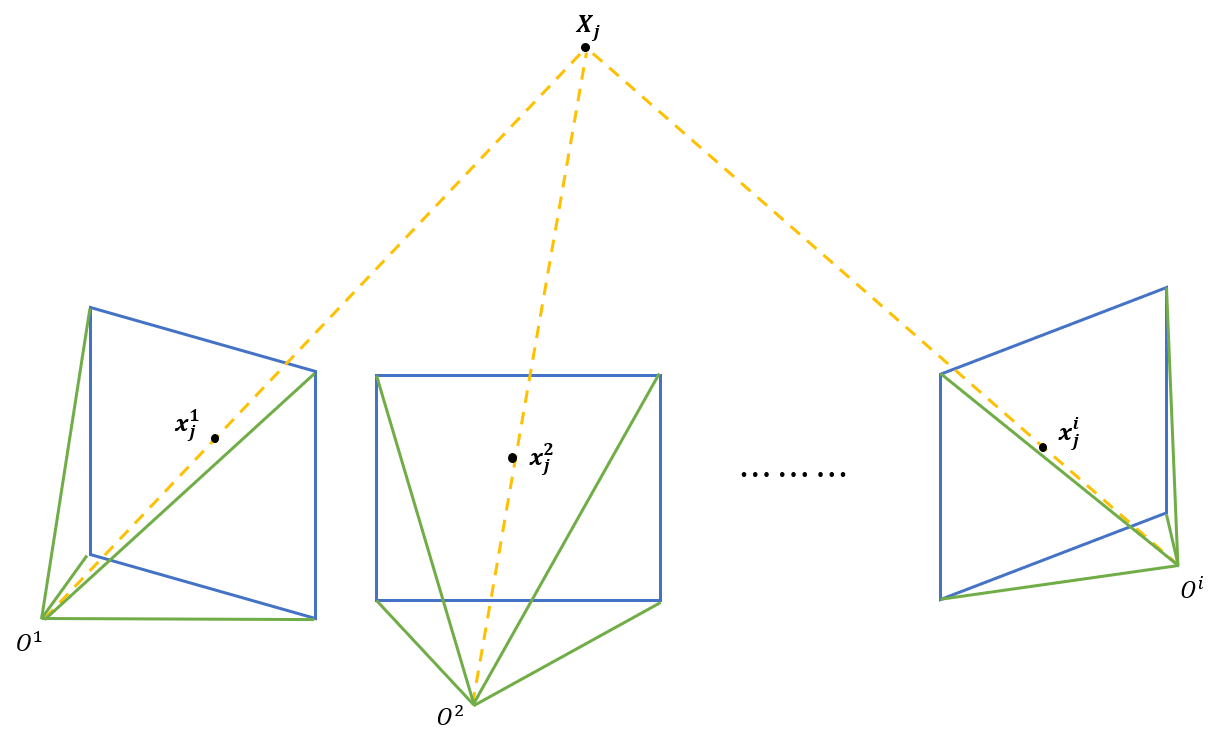
\includegraphics[width=0.8\linewidth]{duomu}
		\caption{多目定位原理图示}
		\label{duomu}
	\end{figure}
	
	根据上述讨论,有等式
	\begin{equation}
		\begin{aligned}
			{\bm x^i_j} = {\bm M_j}{\bm Y^i_j} \\
			{\bm Y^i_j} = {\bm R^i}{\bm X_j} + {\bm T^i}
		\end{aligned}
	\end{equation}
	其中 ${\bm M} = {\bm K^{-1}}$,可以将两个式中合并为一个如式 \ref{eq6}
	\begin{equation}
		{\bm x^i_j} = {\bm M_j}{\bm R^i}{\bm X_j} + {\bm M_j}{\bm T^i}
		\label{eq6}
	\end{equation}
	在考虑误差的情况下,计算式 \ref{eq6} 与实际值 ${\bm x^i_j}$ 可能有所差别,我们的目标就是将误差值最小化,即原问题可转化为非线性规划问题如式 \ref{eq7}
	\begin{equation}
		\min\sum_{i}\sum_{j}({\bm x^i_j} - {\bm M_j}{\bm R^i}{\bm X_j} + {\bm M_j}{\bm T^i})^2
		\label{eq7}
	\end{equation}
	通过上一节方法,对 $R_i, T_i$ 进行标定,即根据若干已知世界坐标系下的点,求解出每个相机坐标系与世界坐标系的变换关系,求解出 $R_i, T_i$ 的值,又由于 ${\bm M_j}$ 实际上是与相机坐标系下 $z$ 有关的矩阵,而 $z$ 与世界坐标系下 $Z$ 的变换关系已经确定,则可以将 ${\bm M_j}$ 看做是只与与世界坐标系下 ${\bm X_j}$ 有关的矩阵,故目标函数中的未知数只有 ${\bm X_j}$,故可以求解该优化问题得到世界坐标系下的点 ${\bm X_j}$。
	\subsection{内部参数标定}
	虽然我们已经假设相机内部不存在误差,但实际上,可以通过一些其他的手段(如实验等)来获得刻画相机特征的一些参数,如成像平面上相邻像素中心的横向与纵向距离、像平面中心的偏移和镜头的非线性畸变参数等,确定数码相机这些内部参数的过程称为相机内部参数标定。得到这些参数后就可对图像数据进行适当的校正,小孔成像原理就正确无误了。
	
	假设实际拍摄图片为 $J$,而使用小孔成像原理计算得到的图片为 $P$,他们之间存在关系
	\begin{equation}
		{\bm P} = {\bm A}{\bm J}
		\label{eq10}
	\end{equation}
	其中矩阵 $\bm A$ 就被称为相机的内部参数矩阵,只需要对于实空间的物品分别使用相机实际拍摄与小孔成像原理计算得到图像矩阵 $P, J$,即可通过式 \ref{10} 计算出相机内部参数矩阵 ${\bm A}$,对于同一个相机来说,内部参数矩阵是确定的,所以在整个过程中只需要计算一次 ${\bm A}$即可。
	\subsection{外部参数标定}
	\subsubsection{靶标及其像}
	标定时,在一块平板上画若干个点,将平板置于适当位置,同时用已安装好的两部相机摄影,分别得到这些点在相片中的位置,利用这两组像点的关系就可求得这两部相机的相对位置。然而无论在物平面上还是在像平面上,人们都无法直接得到没有几何尺寸的“点”。实际的做法是在物平面上画若干个圆,称为靶标,如图 \ref{babiao} 所示,它们的圆心就是几何的点了。
	\begin{figure}[H]
		\begin{minipage}{0.5\linewidth}
			\centering
			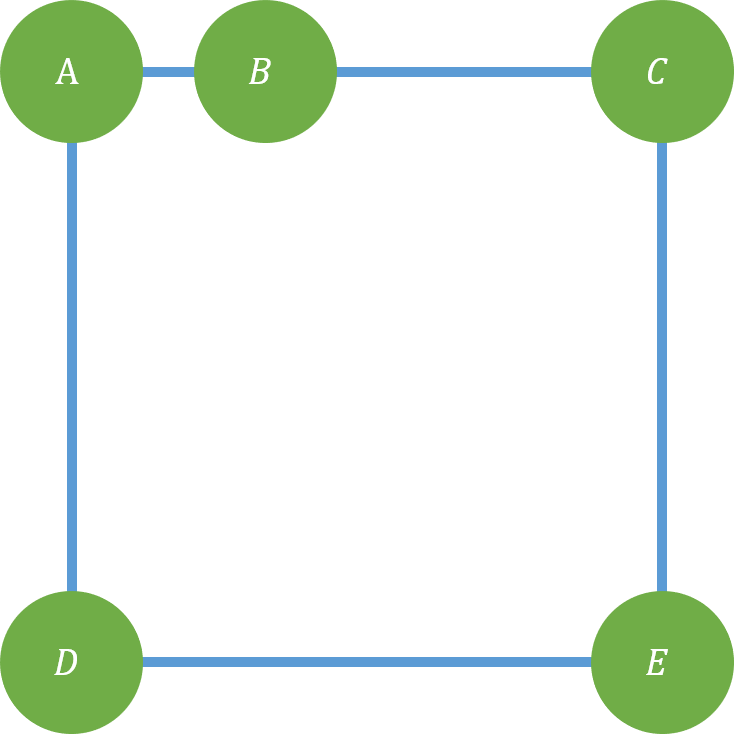
\includegraphics[width=0.7\linewidth]{babiao}
			\caption{靶标}
			\label{babiao}
		\end{minipage}
		\begin{minipage}{0.5\linewidth}
			\centering
			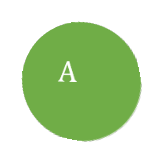
\includegraphics[width=0.25\linewidth]{babiao_A_change}
			\caption{畸变图形}
			\label{babiao_A_change}
		\end{minipage}
	\end{figure}
	
	但由于靶标平面一般并不平行于相机的像平面,靶标上圆的像一般会变形,如图 \ref{babiao_A_change} 所示,因此必须精确地找到照片中圆心的像。
	
	一种可以采用的近似方法是求像的形心,将其作为圆心的像。但是实际上,对某些情形,特别是在靶标平面相对像平面倾斜度较大时,这种方法的误差较大。所以有必要寻找一种新的更精确的求圆心像的方法,取代求形心的方法,在此基础上进行标定,以获得更好的外部参数标定效果。
	
	例如,对一部相机摄得靶标的像由图 \ref{babiao_change}所示.
	
	首先利用图像处理软件对图像进行预处理,提取各个圆的像的边界,结果如图 \ref{babiao_change1}
	\begin{figure}[H]
		\begin{minipage}{0.5\linewidth}
			\centering
			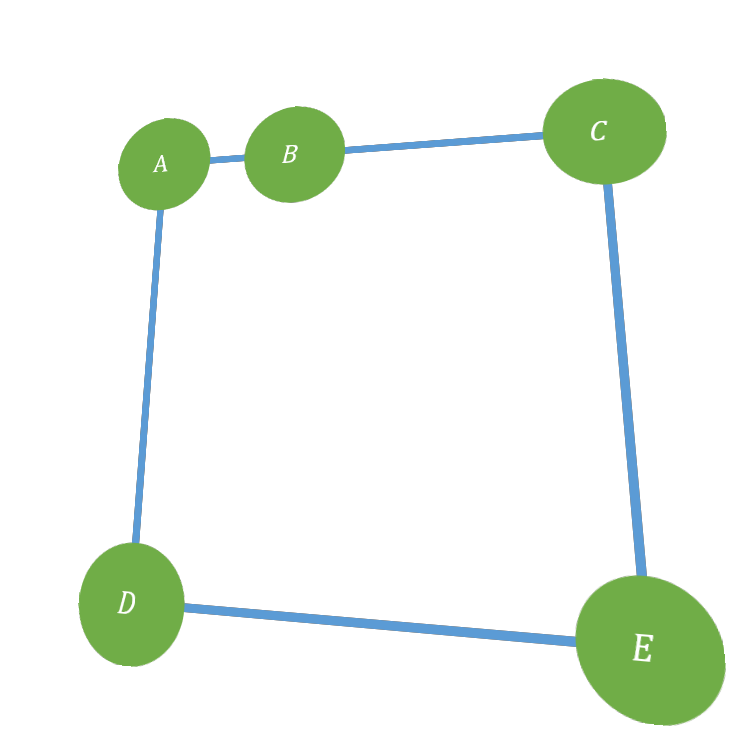
\includegraphics[width=0.7\linewidth]{babiao_change}
			\caption{靶标像}
			\label{babiao_change}
		\end{minipage}
		\begin{minipage}{0.5\linewidth}
			\centering
			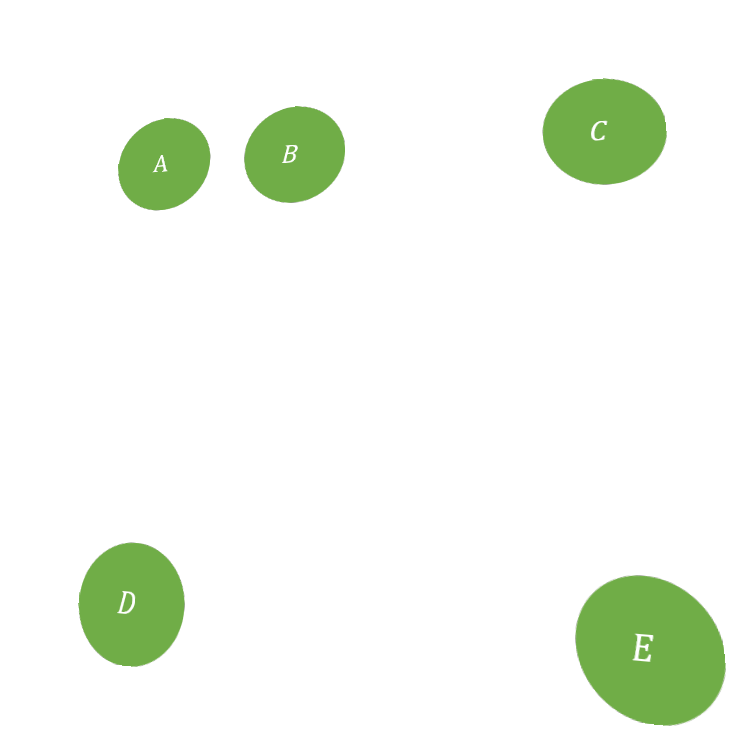
\includegraphics[width=0.7\linewidth]{babiao_change1}
			\caption{提取靶标像边界}
			\label{babiao_change1}
		\end{minipage}
	\end{figure}
	\subsubsection{公切线方法}
	不难证明,变换 \ref{eq1} 将空间的直线变换为像平面的直线,亦即直线的像仍为直线,而圆的像为椭圆.然而,圆心的像一般不是像椭圆的中心。
	
	由于通过成像变换,空间直线变换成像平面上的直线,因此两直线的交点必然映射为两条像直线的交点,另外还可以证明,平面上圆的切线切点映射为相应椭圆的切点.根据这样的分析,我们就可以用作公切线的方法求出各圆圆心像的坐标.例如,分别称圆 $A, B, C, D, E$ 的像为椭圆 $A'$,椭圆 $B‘$,等。作椭圆 $A'$,椭圆 $B'$ 椭圆 $C'$ 的两条外公切线,与椭圆 $A'$ 相切于 $M$ 和 $M'$;再作椭圆 $A'$ 与椭圆 $D'$ 的两条外公切线,与椭圆 $A'$ 相切于 $N$ 和 $N'$ 那么,显然 $MM$ 和 $NN'$ 分别是椭圆 $A'$ 的两条直径的像,它们的交点 $A'$ 就是圆 $A$ 的圆心 $A$ 的像,如图 \ref{babiao_gongqiexian},类似地我们可以求得其余 4 个圆圆心的像的坐标。
	\begin{figure}[H]
		\centering
		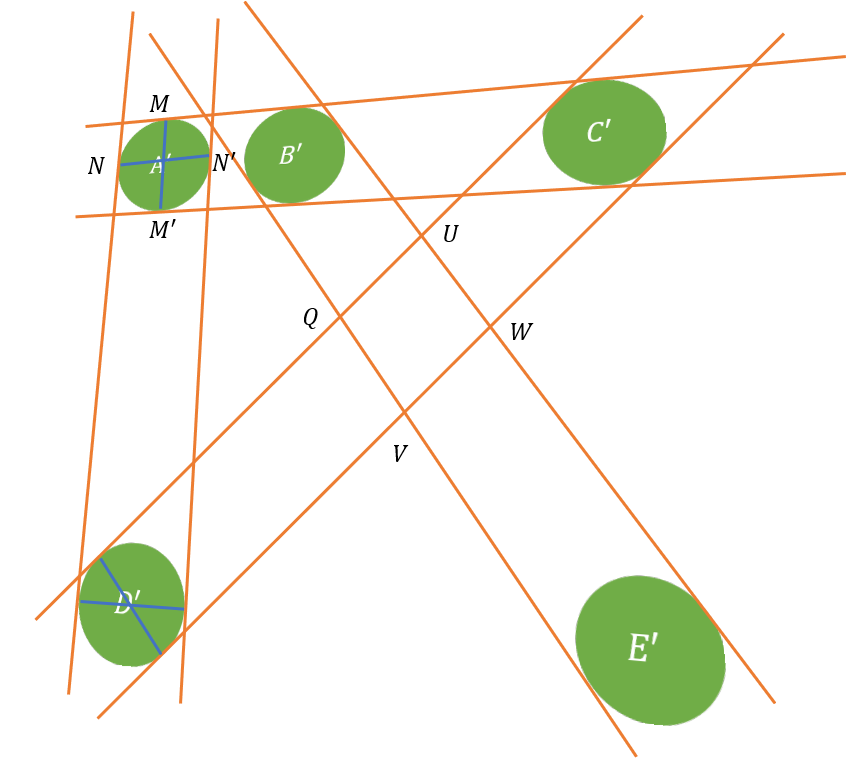
\includegraphics[width=0.6\linewidth]{babiao_gongqiexian}
		\caption{公切线方法图示}
		\label{babiao_gongqiexian}
	\end{figure}
	
	不仅如此,我们还可以利用求其他公切线的交点,得到更多的靶标上已知点的像的坐标,如图 \ref{babiao_gongqiexian} 中的 $Q, U, V, W$ 等。
	
	但是,如果直接对椭圆边界的像素点采用离散的方法求切线和切点会带来较大的误差.比较精确的方法是利用获得的椭圆边界离散点拟合出椭圆方程的表达式,然后用解析方法求切点和公切线,再求出相应的交点。
	\subsubsection{最优化方法}
	求靶标中圆心像的另一种方法是解非线性方程组或将其转化为相应的优化问题,也被称为优化方法。
	
	设在相机坐标系下靶标平面 $D$ 的平面方程为
	\begin{equation}
		ax +by + cz -p = 0
	\end{equation}
	其中 $a, b, c$ 为平面法线的方向余弦,满足 $a^2 + b^2 + c^2 = 1$。设靶标上某圆的圆心坐标为 ${\bm Y_0} = (x_0, y_0, z_0)$,半径为 $R$,圆上任意一点坐标为 ${\bm Y} = (x, y, z)$,在像素坐标系下为 ${\bm x} = (u, v, f)$,由式 \ref{eq1},且点 ${\bm Y}$ 落在平面 $D$ 上,应有
	\begin{equation}
		\frac{z}{f}(au + bv + cf) - p = 0
	\end{equation}
	将 $x, y, z$ 使用 $u, v, f$ 表示,得到
	\begin{equation}
		\left\lbrace
		\begin{aligned}
			x = \frac{pu}{au + bv + cf} \\
			y = \frac{pv}{au + bv + cf} \\
			z = \frac{pf}{au + bv + cf}
		\end{aligned}
		\right.
	\end{equation}
	令 $l = au + bv + cf$,由于 ${\bm x}$ 落在圆周上,故有
	\begin{equation}
		\left(\frac{p}{l}{\bm x} - {\bm Y} \right)^2 = R^2
	\end{equation}
	
	我们可以很容易得到像素平面上椭圆边界上若干点的坐标 ${\bm x_j}, \ j = 1, 2, \dots, n$,可以令 $l_j = au_j + bv_j + cf$,当 $n$ 足够大时,根据约束条件 \ref{eq8} 可以求出 $(a, b, c, p, x_0, y_0, z_0)$。
	\begin{equation}
		s.t.\left\lbrace
		\begin{aligned}
			&\left(\frac{p}{l_j}u_j - x_0 \right)^2 + \left(\frac{p}{l_j}v_j - y_0 \right)^2 + \left(\frac{p}{l_j}f - z_0 \right)^2= R^2 \\
			&a^2 + b^2 + c^2 = 1 \\
			&ax_0 + by_0 + cz_0 = p
		\end{aligned}
		\right.
		\label{eq8}
	\end{equation}
	当然,在实际求解过程中,总会存在很多误差,所以可以将问题转化为最优化问题,目标函数即为计算值与精确值的误差,即式 \ref{eq9}
	\begin{equation}
		\min\sum_{j}\left[ \left(\frac{p}{l_j}u_j - x_0 \right)^2 + \left(\frac{p}{l_j}v_j - y_0 \right)^2 + \left(\frac{p}{l_j}f - z_0 \right)^2 - R^2 \right]^2
		\label{eq9}
	\end{equation}
	在求得 $\bm Y$ 之后,即可用式 \ref{eq1} 求出圆心 ${\bm x_0}$ 的像素坐标。
	\section{模型实现及结果}
	\section{总结}
	
\end{sloppypar}
	\begin{thebibliography}{99}
		\bibitem{1} 姜启源,谢金星,叶俊,数学模型,北京:高等教育出版社,2005.
		\bibitem{2} 徐萃薇,孙绳武,计算方法引论,北京:高等教育出版社,2005.
		\bibitem{3} 谭永基,蔡志杰,数学模型,上海:复旦大学出版社,2019.
		\bibitem{4} 周志华,机器学习,北京:清华大学出版社. 2016.
		\bibitem{5} 李航. 统计学习方法,北京:清华大学出版社. 2012.
		\bibitem{6} 刘启军,曾庆,Logistic回归模型及其研究进展[J].预防医学情报杂志,2002,18(5):3.
		\bibitem{7} 方匡南,吴见彬,朱建平,谢邦昌,随机森林方法研究综述[J].统计与信息论坛,2011,26(3):32-38.
		\bibitem{8} 刘方园,王水花,张煜东,支持向量机模型与应用综述[J].计算机系统应用,2018,27(4):1–9.
	\end{thebibliography}

\end{document}
